\documentclass{book} 
\usepackage[top=3cm,right=3.5cm,bottom=3cm,left=3cm]{geometry}
\renewcommand{\baselinestretch}{1.7}
\usepackage{graphicx}
\parindent=8pt
\begin{document}
page $193$\\\\\\
results and that presented in previous articles. You will also likely unant to consult with colleagues to judge the bias for and against e-iournals in your affiliated institution. Finally, bear in mind that the enhanced accessibility of electronic distribution will send a signal to readers that you are willing and able to take an academic chance and strike one small blow for accessibility by publishing electronically.\\
\textbf{How Does One Locate Prospective e-Journals?}\par 
 E-journals can be located using the large subject directories such as Yahoo! Or Lycos. A January, 2002 search of Yahoo! provides links to 205 electronic journals in all subject areas. Stanford University library (http://www.sul.stanford.edu/collect/eiourns .html\# subj) provides a specialized listing and access to many of the most popular e-journals that are distributed either from the Web or via email. We think you will be delightfully surprised by the quality of many of these e-iournals and will likely seriously consider sending your work for dissemination via this means.\\
\textbf{DISSEMINATION THROUGH THE POPULAR PRESS}\par  
Similar to peer reviewed publications, many opportunities exist for publishing in the popular press in both paper and online formats. Publishing in the non-peer-reviewed popular press does not have the academic prestige ofa peer-reviewed publication, but may, in the long run, be more effective at disseminating the results of your e-research. Publishing in the popular press has a number of advantages over scholarly peer-reviewed journals. First, the review process is generally much faster and often consists of only proofreading for grammatical errors by an editor. Second, your production may get much wider distribution than the often-limited circulation lists of many academic publications. This wider distribution of your research outcomes may result in more tangible connections and opportunities across a wider set Of readers. Third, you may be paid for your efforts!\par 
The list of online publications is long and continually expanding. Unfortunately many Net-based publications are experimental. and too many are short-lived. A search Of popular directories such as Yahoo! reveals a host of online publications, usually catalogued under each Of the maior subject categories. Many of these sites attempt to provide a two-way communication flow between authors and readers or even go so far as to attempt to create a virtual community based on the published articles. For example eserver (http://eserver.org/) provides access to literary, artistic, and rhetorical works from over 200 scholars organized into forty-two collections. As a cooperative of producers, eserver "provides a forum where your project can receive feedback and assis- tance from our members and when you're ready, working with one of our collection editors, you can publish to a worldwide audience" (eserver.org homepage, 2001).\par 
It is often desirable for an e-researcher to publish at least two versions of their results: one for the specific target audience who paid for or inspired the research (often contract, employment, or educational obligation) and a second, more popular, version\newpage
page $194$\\\\\\
that is designed for a more general audience. The Net provides ideal venues for this later publication.\par 
\textbf{Dissemination through a Web Site}\par 
 Creating an e-researcher Web site is likely the most cost-effective means to distribute the results of your research. Finding a server and developing and maintaining Web sites is covered in more detail On this book's accompanying Web site where we discuss ways in which a Web site can be used for promotion, gathering data, and other tasks besides dissemination of results. We do however, wish to highlight one critical issue related to dissemination through a public Web site. Are e-researchers able to disseminate their own articles via their Own Web site? The answer to this question may seem blatantly obvious: of course. Or is it an obvious answer? In fact, when e-researchers do develop their own Web sites, many encounter a major problem if they have previously published the results in other academic journals. Often, as a condition of publication, authors are requested to relinquish their copyright ownership of the article to the publisher of the scholarly journal, edited book, or other format of publication. Once authors relinquish this right, they are not entitled to further disseminate their work even on their own Web site. This may seem unfair and an example of excessive control on the part of the publishers. However, publishers have to protect their readership and if the information is freely available on the author's Web site, they may not sell as many subscriptions to their journals. They also note that they have real costs associated not only with publication and distribution, but also those associated the with editing and the peer-review process. Of course, at a certain point in time sales of the particular issue of the journal come to an end. At this point promotion of the journal, through noting the source of the article's original publication, becomes more likely than loss of sales, so publishers eventually either support or conveniently turn a blind eye to copies of articles to which they own copyright appearing on authors' dissemination sites. The prestigious American Psychology Association (APA) recently formalized their policy in regard to self-dissemination Of authors' work as follows:\par 
Authors of articles appearing in APA copyrighted journals may put up on their personal Web sites the final draft copies of their manuscripts three years After publication. Please consult other publishers and the publishers of APA division publications for their policies (http://www.apa.org/journals/pusting.html).\par 
In our experience. we have sought and usually receive permission from publishers to place copies of our articles on our Web sites long before the three year limit set by the APA. However, this issue reinforces the value of publishing in online journals, so that a direct link can be created from any Web site, providing full access Vo the complete article.\par 
The screen shot in Figure 13.2 is an example of the dissemination site created by a research team led by one of the authors (Anderson) of this book for dissemination of results. We have tried to keep the main page rather free of clutter, but emphasize our affiliation (via the logo at bottom left) with a well known university. We are disseminating\newpage
\begin{figure}
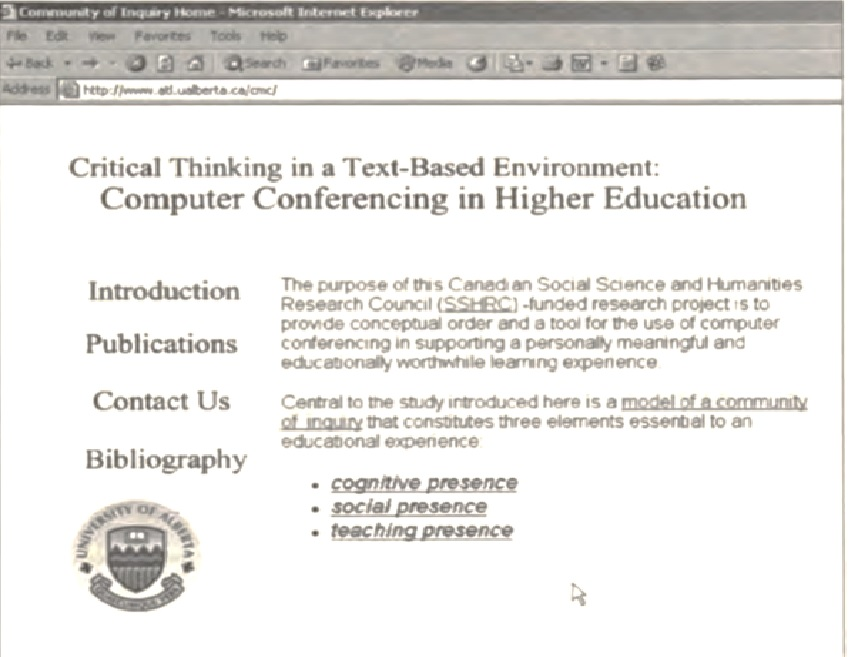
\includegraphics[width=\textwidth]{pic.jpg}
\caption{\textbf{FIGURE 13.2}  Dissemination Site}
\end{figure}
most of the publications from this project after obtaining permission from the journal publications in which they originally appeared. We provide abstracts in HTML format with the complete articles available for download in PDF format. Laura LaMonica's Web site (see Figure 13.3) is an attractive homepage that distributes information about her as well as the results of her latest research. The site thus serves to promote her, acquaint the interested reader further as to her varied interests and experiences, and promote an important research project.\\
\textbf{DISSEMINATION THROUGH EMAIL LISTS OR USENET GROUPS}\par  Topic-specific mailing lists and Usenet groups are often excellent avenues by which you may alert many potential consumers of your research. However, there are a variety of
\end{document}